\documentclass[a4paper,12pt, oneside]{book}

% \usepackage{fullpage}
\usepackage[italian]{babel}
\usepackage[utf8]{inputenc}
\usepackage{amssymb}
\usepackage{amsthm}
\usepackage{graphics}
\usepackage{amsfonts}
\usepackage{listings}
\usepackage{amsmath}
\usepackage{amstext}
\usepackage{engrec}
\usepackage{rotating}
\usepackage[safe,extra]{tipa}
\usepackage{showkeys}
\usepackage{multirow}
\usepackage{hyperref}
\usepackage{mathtools}
\usepackage{microtype}
\usepackage{enumerate}
\usepackage{braket}
\usepackage{marginnote}
\usepackage{pgfplots}
\usepackage{cancel}
\usepackage{polynom}
\usepackage{booktabs}
\usepackage{enumitem}
\usepackage{framed}
\usepackage{algorithm}
\usepackage{algpseudocode}
\usepackage{pdfpages}
\usepackage{pgfplots}
\usepackage[cache=false]{minted}

\usepackage[usenames,dvipsnames]{pstricks}
\usepackage{epsfig}
\usepackage{pst-grad} % For gradients
\usepackage{pst-plot} % For axes
\usepackage[space]{grffile} % For spaces in paths
\usepackage{etoolbox} % For spaces in paths
\makeatletter % For spaces in paths
\patchcmd\Gread@eps{\@inputcheck#1 }{\@inputcheck"#1"\relax}{}{}
\makeatother

\usepackage{tikz}\usetikzlibrary{er}\tikzset{multi
  attribute /.style={attribute ,double  distance =1.5pt}}\tikzset{derived
  attribute /.style={attribute ,dashed}}\tikzset{total /.style={double
    distance =1.5pt}}\tikzset{every  entity /.style={draw=orange ,
    fill=orange!20}}\tikzset{every  attribute /.style={draw=MediumPurple1,
    fill=MediumPurple1!20}}\tikzset{every
  relationship /.style={draw=Chartreuse2, fill=Chartreuse2!20}}
\newcommand{\key}[1]{\underline{#1}}

\usepackage{fancyhdr}
\pagestyle{fancy}
\fancyhead[LE,RO]{\slshape \rightmark}
\fancyhead[LO,RE]{\slshape \leftmark}
\fancyfoot[C]{\thepage}
\usepackage{tikz}
\usetikzlibrary{automata,positioning}


\title{Assignment 1, Bioinformatica}
\author{Davide Cozzi, 829827}
\date{}

\pgfplotsset{compat=1.13}
\begin{document}
\maketitle

\definecolor{shadecolor}{gray}{0.80}
\setlist{leftmargin = 2cm}
\newtheorem{teorema}{Teorema}
\newtheorem{definizione}{Definizione}
\newtheorem{esempio}{Esempio}
\newtheorem{corollario}{Corollario}
\newtheorem{lemma}{Lemma}
\newtheorem{osservazione}{Osservazione}
\newtheorem{nota}{Nota}
\newtheorem{esercizio}{Esercizio}

\renewcommand{\chaptermark}[1]{%
  \markboth{\chaptername
    \ \thechapter.\ #1}{}}
\renewcommand{\sectionmark}[1]{\markright{\thesection.\ #1}}
\chapter{esercizio 1}
\section{Versione 1}
Si assumano stringhe su $\Sigma=\{a,c,g,t,A,C,G,T\}$ indicizzate a partire dalla
posizione 0, per comodità.\\
L'algoritmo si divide in due parti:
\begin{enumerate}
  \item divisione in ``token'' delle due stringhe. A partire da ogni stringa si
  ottiene un vettore di sottostringhe di uguali caratteri
  \item confronto dei due vettori di sottostringhe
\end{enumerate}
%Assumendo in input le due stringhe $v$ e $w$, rispettivamente di lunghezza $n$ e
%$m$
%, si ha che la costruzione dei due vettori ha costo rispettivamente
%$\mathcal{O}(n)$ e $\mathcal{O}(m)$ mentre
%il confronto, possibile solo se i due vettori prodotti hanno lunghezza uguale
%$l$, è in $\mathcal{O}(l)$. \\
Si procede specificando che:
\begin{itemize}
  \item $length(X)$ restituisce la lunghezza di $X$, che sia una stringa o un
  vettore 
  \item $push(X,Y)$ effettua l'operazione di \texttt{push} di $Y$ nel
  vettore/stringa $X$
  \item $string(Y)$ effettua il cast di $Y$ a \texttt{string}
  \item $Y[i,e]$ specifica la sottostringa di $Y$ che va dall'indice $i$ incluso
  all'indice $e$ incluso
  \item $lowercase(Y)$ porta $Y$ in \textit{lowercase}
\end{itemize}
Si ha quindi la prima parte dell'algoritmo, che effettua la divisione in
``token''.
\newpage
\begin{esempio}
  Vediamo un esempio di input e output della funzione \texttt{Splitter}.
  \begin{itemize}
    \item \textbf{input}: \textit{"aaataaaggggccccctttttttttttttttcc"}
    \item \textbf{output}: \textit{["aaa", "t", "aaa", "gggg", "ccccc",
      "ttttttttttttttt", "cc"]} 
  \end{itemize}
\end{esempio}
Si ha quindi lo pseudocodice:
\begin{algorithm}[H]
  \begin{algorithmic}
    \Function{Splitter}{$s$}
    \State $result \gets \left[\,\,\,\right]$
    \State $n\gets length(s)$
    \State $last\_mismatch \gets 0$
    \If {$n==1$}
    \State $push(result, string(s[0]))$
    \State \textbf{return} $result$
    \EndIf
    \State $tmp \gets ""$
    \For {$i\gets 0$ \textbf{to} $n$}
    \If {$i > 0$ \textbf{and} $s[i-1]\neq s[i]$}
    %\State $tmp \gets s[last\_mismatch, i-1]$
    \State $push(result, tmp)$
    \State $tmp \gets ""$
    %\State $last\_mismatch \gets i$
    \EndIf
    \State $push(tmp, s[i])$
    \If {$i == (n-1)$}
    % \State $tmp \gets s[last\_mismatch, n-1]$
    % \State $push(result, tmp)$
    \State $push(result, tmp)$
    \EndIf
    \EndFor
    \State \textbf{return} $result$
    \EndFunction
  \end{algorithmic}
  \caption{Algoritmo per lo split in ``token'' delle stringhe}
\end{algorithm}
Una volta ottenuto il vettore dei ``token'' delle due sequenze in input basta
confrontare i due vettori.\\
Prima di vedere il confronto si specifica che:
\begin{itemize}
  \item le due sequenze vengono trasformate in \textit{lowercase} per praticità
  \item si assume che le due sequenze non possono essere stringhe vuote
  $\varepsilon$ 
\end{itemize}
Fatte queste assunzioni si può fare ancora un ultima osservazione prima di
procedere con l'algoritmo. Qualora i due vettori prodotti dalla funzione
\texttt{Splitter} fossero di lunghezza diversa allora l'algoritmo non potrà in
nessun caso dire che ci sia stata un'''infezione'' in quanto si assume che non
ci siano né \textit{gaps} né \textit{inserimenti}. In altri termini qualora i
due vettori siano di diversa cardinalità sicuramente, con queste premesse, non è
avvenuta alcuna infezione. Vediamo ora le altre casistiche. Si itera
contemporaneamente sull'elemento i-esimo dei due vettori e:
\begin{itemize}
  \item se i due elementi i-esimi presentano il primo carattere diverso allora,
  date le premesse, si specifica che non può essere avvenuta un'infezione
  \item se i due elementi i-esimi presentano il primo carattere uguale allora si
  procede confrontando i due elementi i-esimi (si assuma $X$ vettore relativo
  alla ``sequenza originale'' e $Y$ vettore relativo alla sequenze che si vuole
  dimostrare l'eventuale infezione):
  \begin{itemize}
    \item se il primo carattere è ``a'' allora la lunghezza di $Y[i]$ deve
    essere minore o uguale a 5 volte quella di $X[i]$, in quanto per ogni ``a''
    in $X[i]$ posso avere al più 5 ``a'' in $Y[i]$
    \item se il primo carattere è ``t'' allora la lunghezza di $Y[i]$ deve
    essere minore o uguale a 10 volte quella di $X[i]$, in quanto per ogni ``t''
    in $X[i]$ posso avere al più 10 ``t'' in $Y[i]$
    \item se il primo carattere è ``c'' o ``g'' allora la lunghezza di $Y[i]$
    deve essere maggiore o uguale di quella di $X[i]$, in quanto per ogni ``c''
    o ``g'' in  in $X[i]$ posso avere un numero indefinito di ``c'' o ``g'' in
    $Y[i]$ 
  \end{itemize}
\end{itemize}
\newpage
Si ha quindi il seguente pseudocodice dell'algoritmo, che ritorna $\top$ o
$\bot$ a seconda che sia possibile che $seq2$ sia una versione infettata di
$seq1$:
\begin{algorithm}[H]
  \begin{algorithmic}
    \Function{CheckInfection}{$seq1,seq2$}
    \If{$length(seq1) == 0$ \textbf{or} $length(seq2)==0$}
    \State \textbf{return} $\bot$
    \EndIf
    \State $vecseq1\gets Splitter(lowercase(seq1))$
    \State $vecseq2\gets Splitter(lowercase(seq2))$
    \State $check \gets \top$
    \If {$length(vecseq1)\neq length(vecseq2)$}
    \State \textbf{return} $\bot$
    \EndIf
    \State $j \gets length(vecseq1)$
    \For {$i\gets 0$ \textbf{to} $j$}
    \If {$vecseq1[i][0] \neq vecseq2[i][0]$}
    \State \textbf{return} $\bot$
    \EndIf
    \If {$vecseq1[i][0]==\,'a'$}
    \State $check \gets (length(vecseq2[i]) \leq 5\cdot length(vecseq1[i]))$
    \ElsIf {$vecseq1[i][0]==\,'t'$}
    \State $check \gets (length(vecseq2[i]) \leq 10\cdot length(vecseq1[i]))$
    \Else
    \State $check \gets (length(vecseq2[i]) \geq length(vecseq1[i]))$
    \EndIf
    \EndFor
    \State \textbf{return} $check$
    \EndFunction
  \end{algorithmic}
  \caption{algoritmo di verifica dell'infezione}
\end{algorithm}
\begin{esempio}
  Qualche esempio:
  \begin{itemize}
    \item \textbf{input}: "ATAGCTC" e \\"AAATAAAGGGGCCCCCTTTTTTTCC" 
    \item \textbf{output}: $\top$
  \end{itemize}
  infatti (si usano i colori per rappresentare i vari ``token'' dei vettori):
  \begin{center}
    \color{blue}A\color{green}T\color{blue}A\color{red}G\color{yellow}C\color{green}T\color{yellow}C\\ 
    \color{blue}AAA\color{green}T\color{blue}AAA\color{red}GGGG\color{yellow}CCCCC\color{green}TTTTTTT\color{yellow}CC
  \end{center}
  Avendo che tutti i vincoli sono rispettati.
  \newpage
  D'altro canto vediamo un esempio in cui non si può dire di avere una
  mutazione: 
  \begin{itemize}
    \item \textbf{input}: "ATAGCTC" e \\"AAATAAAAAAGGGGCCCCCTTTTTTTCC" 
    \item \textbf{output}: $\bot$
  \end{itemize}
  infatti (si usano i colori per rappresentare i vari ``token'' dei vettori):
  \begin{center}
    \color{blue}A\color{green}T\color{blue}A\color{red}G\color{yellow}C\color{green}T\color{yellow}C\\ 
    \color{blue}AAA\color{green}T\color{blue}AAAAAA\color{red}GGGG\color{yellow}CCCCC\color{green}TTTTTTT\color{yellow}CC
  \end{center}
  Avendo che il terzo ``token'' della prima stringa è {\color{blue}A} mentre
  quello della seconda stringa è {\color{blue}AAAAAA}, avendo che viene rotto il
  vincolo per il quale per ogni $A$ posso avere al più 5 $A$ nella mutazione.\\
  Un altro esempio in cui non si può dire di avere una
  mutazione è: 
  \begin{itemize}
    \item \textbf{input}: "ATAGCTC" e \\"AAACCTAAAAAAGGGGCCCCCTTTTTTT" 
    \item \textbf{output}: $\bot$
  \end{itemize}
   infatti (si usano i colori per rappresentare i vari ``token'' dei vettori):
  \begin{center}
    \color{blue}A\color{green}T\color{blue}A\color{red}G\color{yellow}C\color{green}T\color{yellow}C\\ 
    \color{blue}AAA\color{yellow}CC\color{green}T\color{blue}AAAAAA\color{red}GGGG\color{yellow}CCCCC\color{green}TTTTTTT
  \end{center}
  In quanto i due secondi ``token'', {\color{green}T} e {\color{yellow}CC},
  corrispondono a caratteri diversi.
\end{esempio}
\newpage
\section{Versione 2}
Si assumano stringhe su $\Sigma=\{a,c,g,t,A,C,G,T\}$ indicizzate a partire dalla
posizione 0, per comodità.\\
Indico anche una versione intuitivamente più semplice. In questo caso si scorre
la sequenze che si suppone essere 
originale, tenendo conto dei caratteri uguali ripetuti. Appena si ha un cambio
di carattere si verifica se nella sequenza che si vuole dimostrare essere una
mutazione di quella originale si ha una corretta sequenza di caratteri secondo
la specifica.\\
Si ha che:
\begin{itemize}
  \item per comodità le sequenze sono riportate in lowercase e si assume che, in
  presenza di anche solo una sequenza nulla, l'algoritmo restituisce $\bot$
  \item \texttt{seq1} e \texttt{seq2} sono rispettivamente la sequenza originale
  al sequenza che si vuole dimostrare essere la mutazione
  \item \texttt{co} e \texttt{cm} sono le variabili che ogni volta
  accumulano il conteggio dei caratteri uguali consecutivi rispettivamente sulla
  sequenza originale e su quella che si suppone mutata
  \item $i$ e $j$ sono rispettivamente gli indici per la prima e per la seconda
  sequenza 
\end{itemize}
In poche parole si itera sulla sequenza originale, aggiornando di volta in volta
il contatore relativo finché si ha lo stesso carattere. Nel momento in cui si ha
un cambiamento o si è arrivato all'ultimo carattere della sequenza si ferma il
conteggio e si verifica il conteggio sulla seconda sequenza (anche in questo
caso facendo attenzione a non andare \textit{out of bounds}). Qualora la seconda
sequenza presenti, all'indice a cui si è arrivati con l'algoritmo, un carattere
diverso da quello della prima si può restituire $\bot$. Controllando la
seconda sequenza si aggiorna il rispettivo contatore e l'indice. Una volta che
anche sulla seconda sequenza si ha un cambio di carattere o si è arrivati alla
fine si confrontano i due contatori secondo le specifiche (ad esempio se nella
stringa originale avevo due ``a'' consecutive ne posso avere al più 10 in quella
che si vuole verificare essere la mutazione). Finito questo controllo si
azzerano i contatori e si verifica che, qualora la sequenza originale sia stata
visitata interamente, anche la seconda sia conclusa. In caso contrario si
restituisce $\bot$.\\
Si ha quindi il seguente pseudocodice.
\begin{algorithm}[H]
  \begin{algorithmic}
    \Function{CheckInfection}{$seq1,seq2$}
    \State $m \gets length(seq1)$
    \State $n \gets length(seq2)$
    \If{$m == 0$ \textbf{or} $n==0$}
    \State \textbf{return} $\bot$
    \EndIf
    \State $seq1\gets lowercase(seq1)$
    \State $seq2\gets lowercase(seq2)$
    \State $co \gets 0$
    \State $cm \gets 0$
    \State $j \gets 0$
    \For {$i\gets 0$ \textbf{to} $m$}
    \State $co \gets co+1$
    \If {$i==n-1$ \textbf{or} $seq1[i]\neq seq[i+1$}
    \If {$seq1[i]\neq seq2[j]$}
    \State \textbf{return} $\bot$
    \EndIf
    \While {$j \neq n-1$ \textbf{and} $seq2[j]==seq2[j+1]$}
    \State $cm \gets cm+1$
    \State $j \gets j+1$
    \EndWhile
    \State $cm \gets cm+1$
    \State $j \gets j+1$
    \If {$seq1[i]==\,'a'$ \textbf{and} $cm \leq 5\cdot co$}
    \State $check \gets \top$
    \ElsIf {$seq1[i]==\,'t'$ \textbf{and} $cm \leq 10\cdot co$}
    \State $check \gets \top$
    \ElsIf {($seq1[i]==\,'c'$ \textbf{or} $seq1[i]==\,'g'$) \textbf{and}
    $cm \geq co$} 
    \State $check \gets \top$
    \Else
    \State  \textbf{return} $\bot$
    \EndIf
    \State $co \gets 0$
    \State $cm \gets 0$
    \If {$i==m-1$ \textbf{and} $j\neq n$}
    \State  \textbf{return} $\bot$
    \EndIf
    \EndIf
    \EndFor
    \State \textbf{return} $check$
    \EndFunction
  \end{algorithmic}
  \caption{algoritmo di verifica dell'infezione, seconda versione}
\end{algorithm}
Dal punto di vista pratico questo secondo algoritmo evita la fase di
preprocessing vista nel primo algoritmo con la funzione
\texttt{Splitter}. Anziché avere a priori le sottostringhe di cui confrontare le
lunghezze tiene conto di volta in volta dei caratteri uguali consecutivi,
confrontando i contatori (motivo per cui anche gli esempi possono essere
riadattati anche a questa seconda versione). Dal
punto di vista computazionale, assumendo che la funzione \texttt{length} abbia
costo lineare si ha in entrambi i casi un tempo quadratico nel caso peggiore,
anche se si potrebbe fare uno studio più approfondito. 
\chapter{Esercizio 2}
\chapter{Esercizio 3}
La \textbf{distanza di Hamming} tra due stringhe, che si assumono di uguale
lunghezza, è 
il numero di indici per i quali i due caratteri associati sulle due stringhe
sono diversi. È quindi un conteggio delle sostituzioni necessarie per passare da
una stringa all'altra.\\
Ipotizzando di voler studiare la distanza di Hamming tra due sequenze tramite la
griglia estesa si può ipotizzare di ragionare solo in termini di una delle due
sequenze, ovvero considerare i pesi degli archi in ottica di una sola delle due
sequenze. Si associano quindi i seguenti pesi:
\begin{itemize}
  \item $w(diagonale)=0$
  \item $w(verticale)=0$
  \item $w(orizzontale)=1$
\end{itemize}
o, in modo speculare se si vuole ragionare sull'altra sequenza:
\begin{itemize}
  \item $w(diagonale)=0$
  \item $w(verticale)=1$
  \item $w(orizzontale)=0$
\end{itemize}
Dove gli archi diagonali rappresentano un match.\\
A questo punto si cerca il cammino di peso minimo che parte dal nodo
\textit{source}, posto in alto a sinistra, e arriva al nodo \textit{sink}, posto
in basso a destra.\\
Prendendo, ad esempio, in input:
\begin{itemize}
  \item AAAGTTC
  \item AAACTTT
\end{itemize}
Si ha un cammino minimo (non l'unico), assumendo costo degli archi in
orizzontale pari a 1 e in verticale pari a 0, del tipo:
\begin{figure}[H]
  \centering
  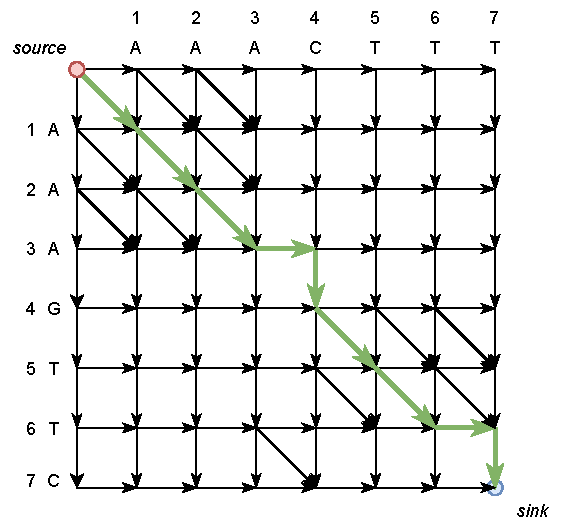
\includegraphics[scale = 1]{img/es3.pdf}
\end{figure}
\noindent
Dove in verde è segnato il cammino minimo scelto. Avendo solo due archi
orizzontali, che ricordiamo avere peso 1 mentre gli altri hanno peso nullo,
possiamo concludere che la distanza di Hamming tra le due stringhe è 
pari a 2.
\chapter{Esercizio 4}
Il problema della \textbf{longest common substring} si pone l'obiettivo di
estrarre, a partire da due stringhe di lunghezza arbitraria, anche non uguale,
la sottostringa, comune ad entrambe, più lunga.\\
Dal punto di vista della griglia si assegnano i seguenti pesi:
\begin{itemize}
  \item $w(diagonale)=1$
  \item $w(verticale)=-1\cdot i$
  \item $w(orizzontale)=-1\cdot j$
\end{itemize}
Dove gli archi diagonali rappresentano un match.\\
\textbf{Qualora si ottenga un valore negativo viene messo 0}.\\
Si ragiona quindi tenendo traccia del valore massimo raggiungo, tenendo traccia,
per una maggior efficienza, anche delle coordinate. Una volta completata la
griglia si avrà che il valore massimo corrisponde al nodo \textit{sink} del
cammino composto dalla più lunga sequenza possibile di archi diagonali
consecutivi. Qualsiasi altra ``operazione'', con archi orizzontali o diagonali,
comporta infatti una perdita di punteggio e ogni volta che un cammino diagonale
termina viene azzerato il punteggio, tramite pesi negativi pesati sugli
indici. Il valore massimo quindi altro non è che 
la lunghezza della \textit{longest common substring}. Sapendo che archi
diagonali corrispondono a match tra le due sequenze si ottiene che tale cammino
corrisponde alla \textit{longest common substring}. \\
Volendo si può scegliere di salvare in un vettore i valori massimi qualora
coincidano, per ottenere eventuali più \textit{longest common substring} qualora
ce ne siano.\\
Per ricostruire la \textit{longest common substring} si parte dal nodo
\textit{sink}, come detto definito dal valore massimo calcolato. Si aggiunge il
carattere corrispondente e si risale tutto il cammino diagonale, aggiungendo di
volta in volta in testa il carattere letto. Ci si ferma quindi quando non si ha
più un nodo il cui punteggio è stato ottenuto tramite un arco diagonale.
\newpage
Vediamo quindi un esempio pratico. Siano date:
\begin{itemize}
  \item AAACGCGCTTTTTCCCAT
  \item AAAGGGGCGCGCTTTTTAAA
\end{itemize}
Si costruisce quindi la griglia e si identifica il cammino diagonale più lungo:
\begin{figure}[H]
  \centering
  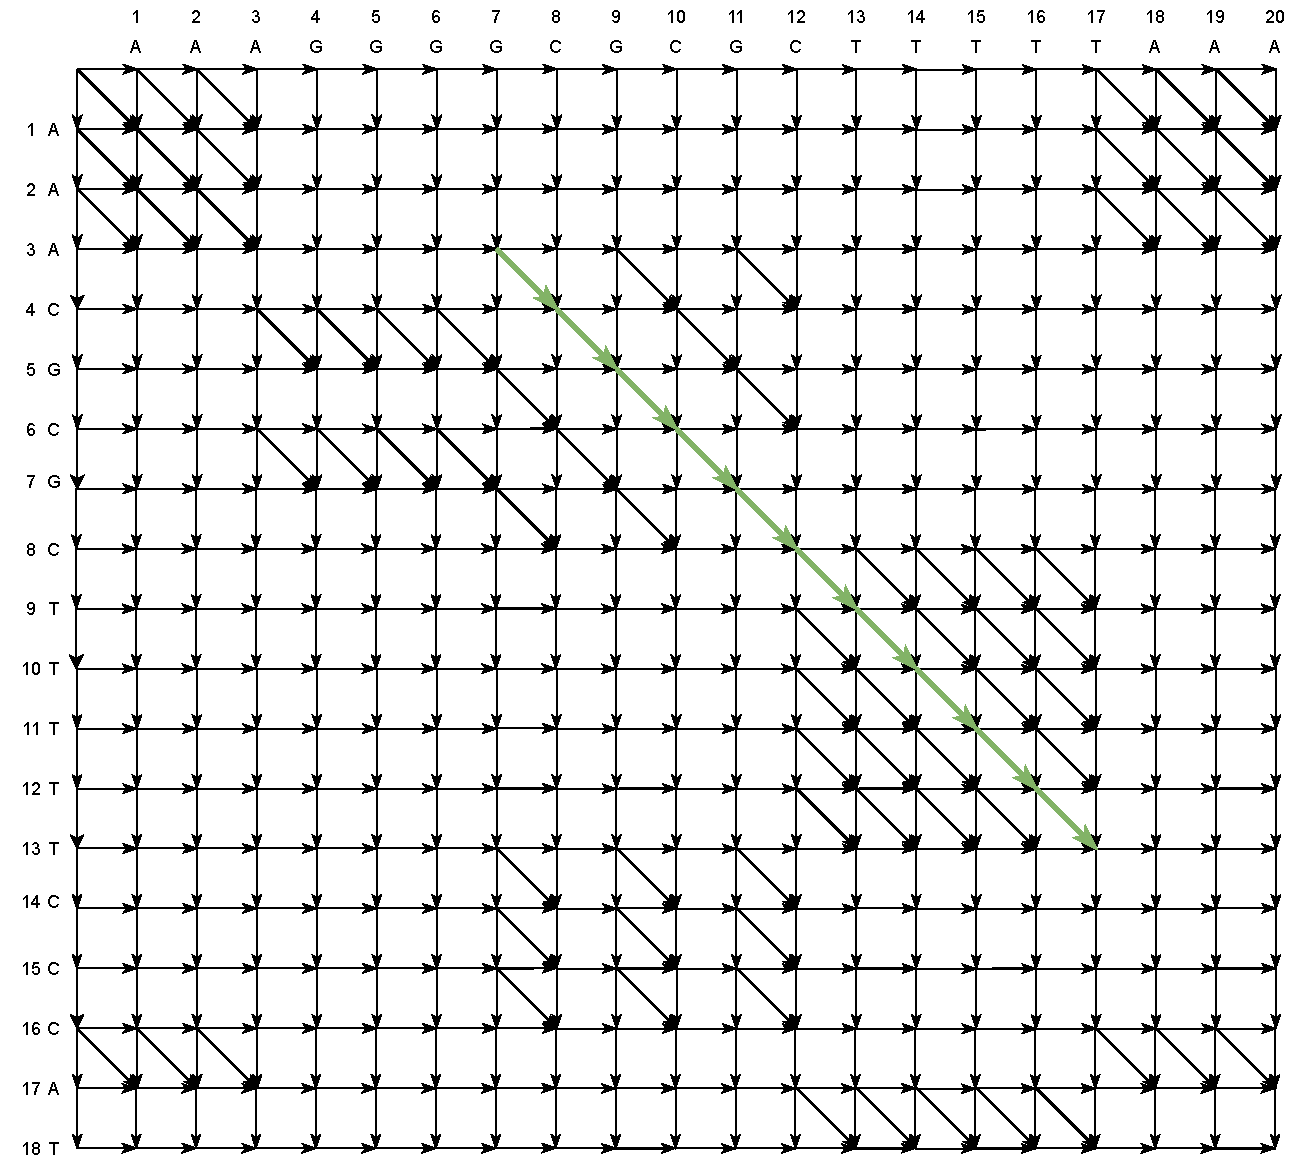
\includegraphics[scale = 0.62]{img/es4.pdf}
\end{figure}
Ricostruendo si ha che tale cammino identifica un massimo pari a 10 e si
ricostruisce: 
\begin{center}
  CGCGCTTTTT
\end{center}
che è appunto la \textit{longest common substring} delle due sequenze in input.
\end{document}

% LocalWords:  sottostringhe sottostringa pseudocodice lowercase
